\documentclass{article}

\usepackage[utf8]{inputenc}
\usepackage[T1]{fontenc}
\usepackage{lipsum}
\usepackage{graphicx}
\usepackage{amsmath}
\usepackage[margin=1in]{geometry}
\usepackage{titlesec}
\usepackage{enumitem}

\titleformat{\section} 
{\LARGE\bfseries}{\thesection}{1em}{}

\titleformat{\subsection} 
{\Large\bfseries}{\thesection}{1em}{}

\begin{document}

\pagestyle{empty}

\section*{Progettazione concettuale} 
\large

La costruzione di uno schema concettuale deve tenere conto di alcune \textbf{proprietà generali} che ne determinano la \textbf{qualità}:
\begin{itemize}[label={-}, leftmargin=1cm]
    \item \textbf{Correttezza}: utilizzo corretto sintattico e semantico dei costrutti del modello E/R
    \item \textbf{Completezza}: rappresentazione di tutti i dati d'interesse descritti nel documento di specifica
\end{itemize}
Per garantire tali proprietà vengono utilizzate diverse \textbf{metodologie di progettazione concettuale}. Alcune di queste possono essere:

\subsection*{Strategie di progettazione}
\large

Il documento di specifica potrebbe essere \textbf{molto complesso} e \textbf{denso di contenuti}. Per costruire il modello E/R si possono utilizzare diverse \textbf{strategie}:
\begin{itemize}[label={-}, leftmargin=1cm]
    \item \textbf{Strategia top-down}: lo schema concettuale viene ottenuto attraverso una \textbf{serie di raffinamenti successivi a partire da uno schema iniziale} molto astratto
    \item \textbf{Strategia bottom-up}: le \textbf{specifiche iniziali sono suddivise in componenti} via via più piccole, ed in un secondo momento \textbf{i vari schemi sono integrati} tra loro
    \item \textbf{Strategia inside-out}: si \textbf{individuano una serie di concetti importanti} e poi si procede a \textbf{partire da questi verso concetti correlati}, con un'estensione a macchia d'olio. E' un caso particolare della strategia \textit{bottom-up}
    \item \textbf{Strategia mista}: si utilizza una combinazione delle strategie precedenti. Si suddivide quindi in diversi step:
    \begin{enumerate}[leftmargin=1cm]
        \item Si individuano i \textbf{concetti principali} o più citati
        \item Si realizza uno \textbf{schema scheletro}
        \item \textbf{Si decompone} lo schema
        \item \textbf{Si raffina} lo schema, si espande e si integra
    \end{enumerate}
    In molti casi pratici di una certa complessità, la strategia mista rappresenta la scelta migliore
\end{itemize}

\subsection*{Pattern di progettazione}
\large

Si parte dal concetto che \textbf{non esiste una rappresentazione univoca delle specifiche}, quindi è meglio attenersi alle \textbf{Regole Concettuali (RC)} del diagramma E/R. Le tre \textit{regole concettuali} sono:
\begin{itemize}[label={-}, leftmargin=1cm]
    \item \textbf{RC1}: se un concetto ha proprietà significative e descrive oggetti con esistenza autonoma, si utilizzano \textbf{Entità}
    \item \textbf{RC2}: se un concetto correla due o più Entità, si utilizzano \textbf{Relazioni}
    \item \textbf{RC3}: se un concetto è un caso particolare dell'altro, si utilizzano \textbf{Generalizzazioni}
\end{itemize}
Esistono molti \textbf{pattern}, ovvero \textbf{soluzioni di problemi ricorrenti}, usati nella progettazione concettuale. Se ne osservino alcuni.\vspace*{14pt}\\
\textit{$Pattern_1$}\\
Concetti di tipo "\textbf{parte di}" attraverso l'utilizzo di \textbf{relazioni uno a molti}.
\begin{center}
    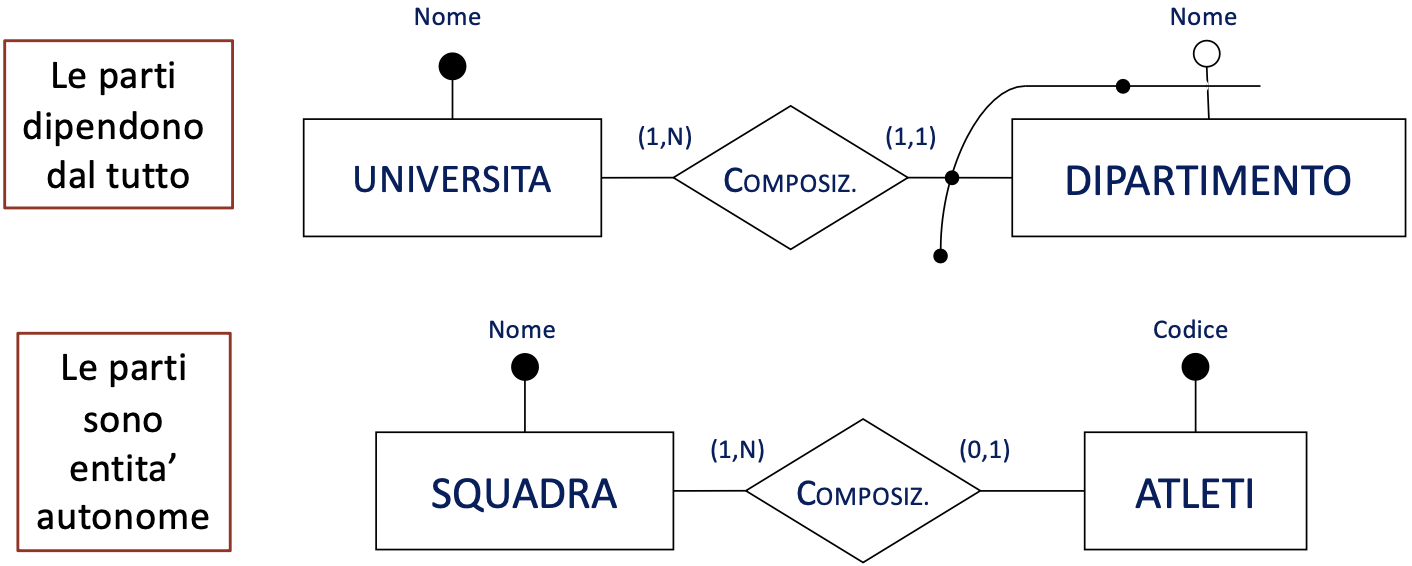
\includegraphics[width=0.55\textwidth]{foto 4.png}
\end{center}
\textit{$Pattern_2$}\\
Introduzione di \textbf{nuove entità} in \textbf{relazioni uno a molti} per la gestione dei duplicati.
\begin{center}
    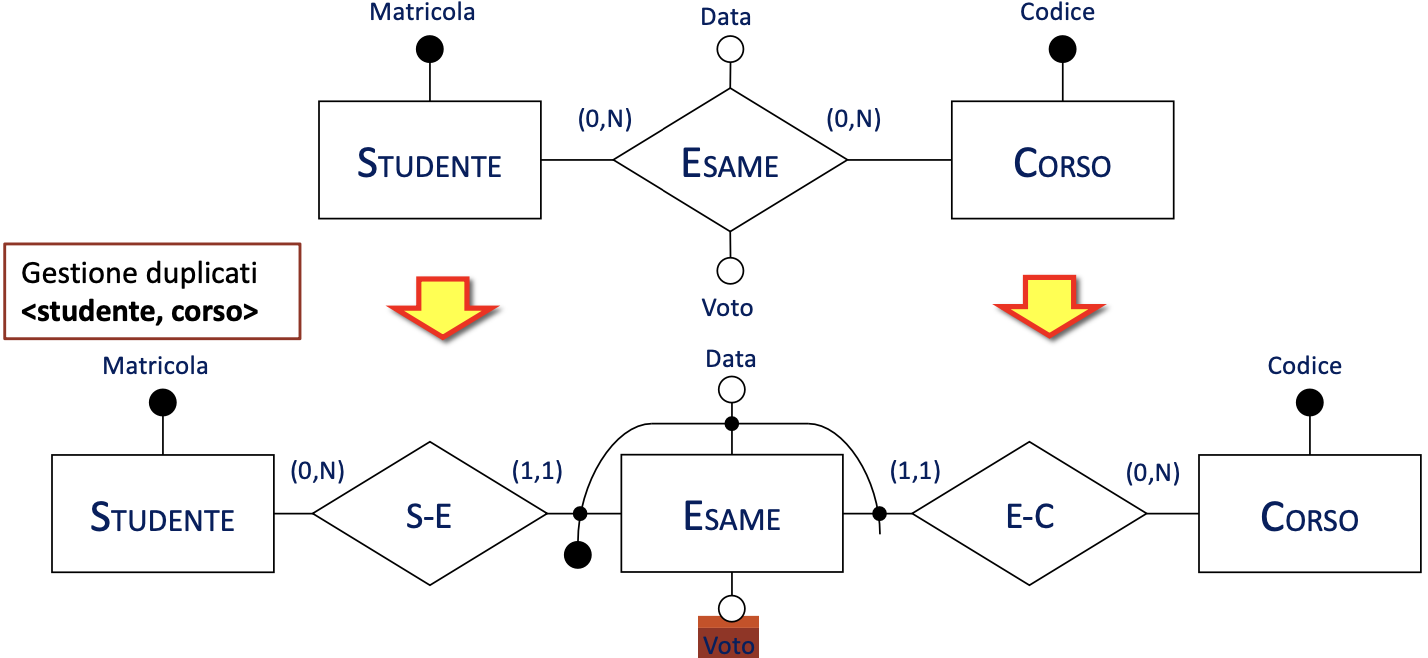
\includegraphics[width=0.6\textwidth]{foto 5.png}
\end{center}
\textit{$Pattern_3$}\\
Utilizzo di \textbf{generalizzazioni} per tenere traccia della \textbf{storia di un concetto}, ossia della sua istanza attuale e di quelle pregresse.
\begin{center}
    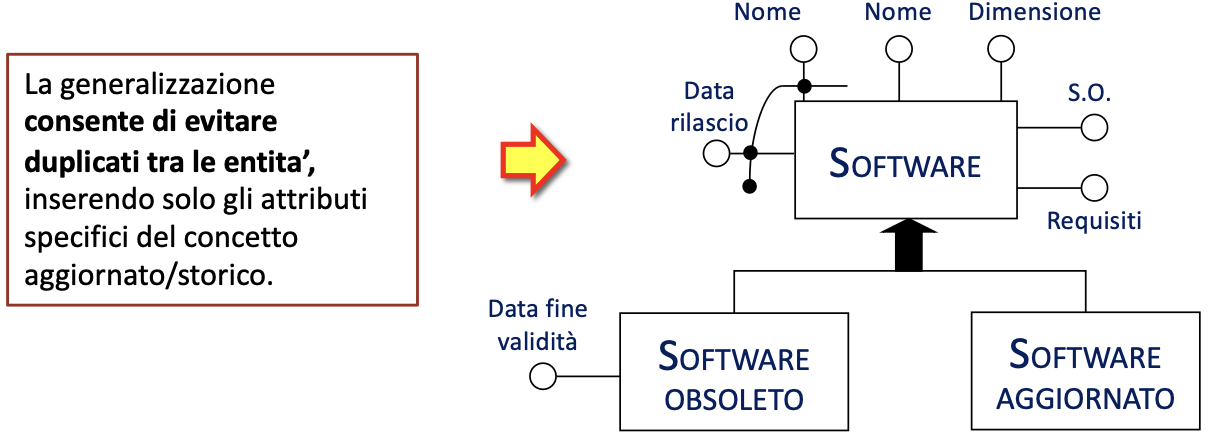
\includegraphics[width=0.6\textwidth]{foto 6.png}
\end{center}
\textit{$Pattern_4$}\\
Utilizzo di \textbf{generalizzazioni} per tenere traccia dell'\textbf{evoluzione nel tempo di un certo concetto}, ossia la creazione di nuove istanze diverse dal concetto originario.
\begin{center}
    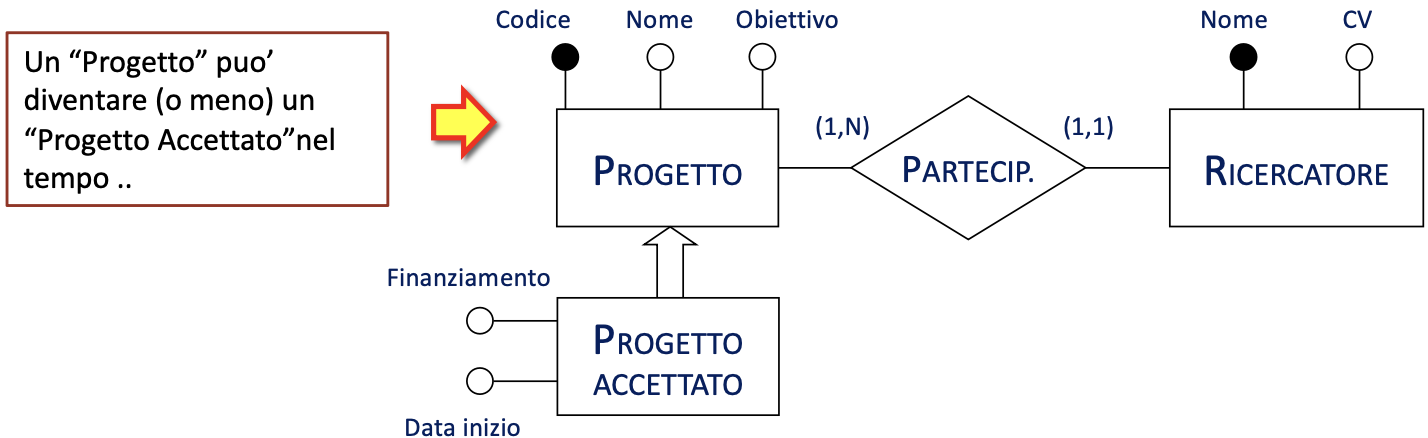
\includegraphics[width=0.6\textwidth]{foto 7.png}
\end{center}

\subsection*{Analisi di prestazione}
\large

Una volta realizzato il modello E/R, è importante analizzarne l'\textbf{efficienza dal punto di vista prestazionale}. Alcuni indici di prestazione possono essere:
\begin{itemize}[label={-}, leftmargin=1cm]
    \item \textbf{Costo operazionale}: numero di entità/associazioni mediamente visitate per implementare una certa operazione sui dati
    \item \textbf{Occupazione di memoria}: spazio di memoria necessario per memorizzare i dati
\end{itemize}
Per poter stimare correttamente l'\textbf{efficienza prestazionale} di uno schema E/R, abbiamo necessità di \textbf{informazioni aggiuntive}.
\begin{center}
    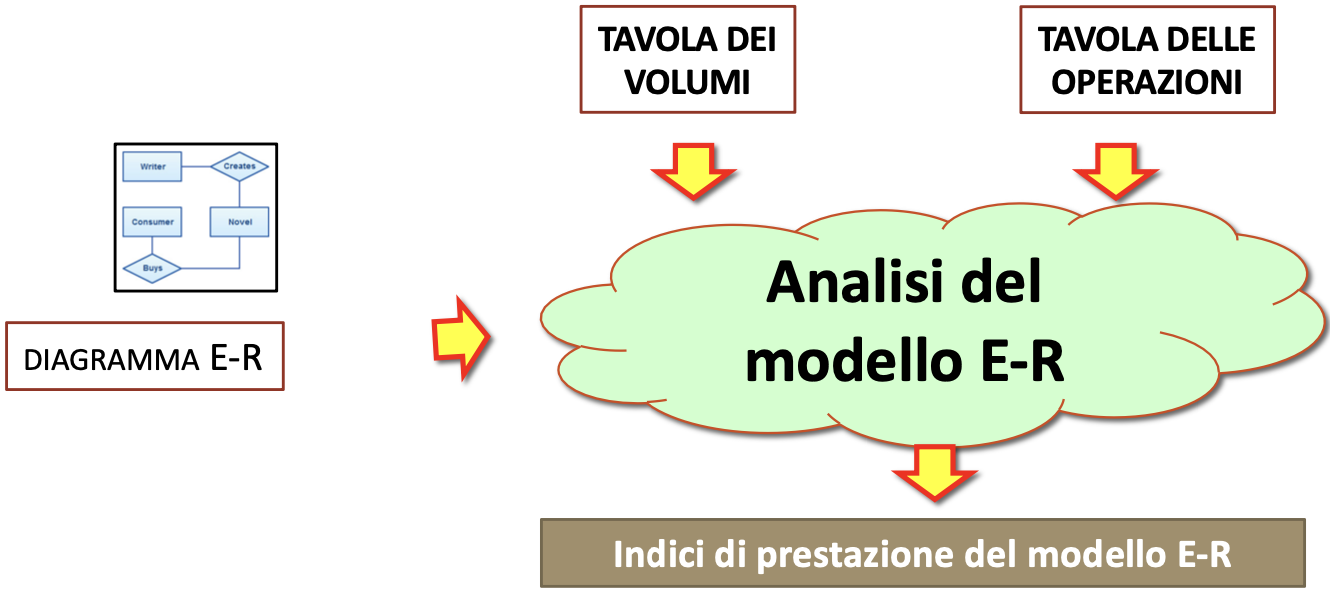
\includegraphics[width=0.6\textwidth]{foto 8.png}
\end{center}
\textit{Tavola dei volumi}\\
La \textbf{tavola dei volumi} fornisce una \textbf{stima del numero di occorrenze entità/relazioni} presenti nel modello E/R. Si osservi un esempio:
\begin{center}
    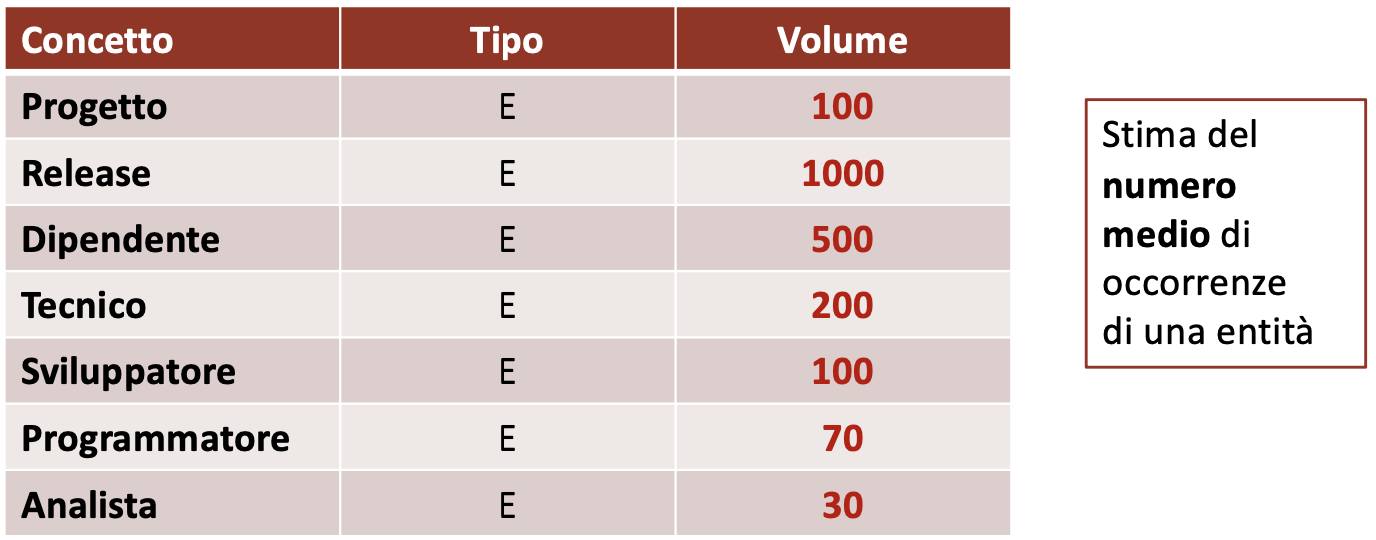
\includegraphics[width=0.6\textwidth]{foto 9.png}
\end{center}
\begin{center}
    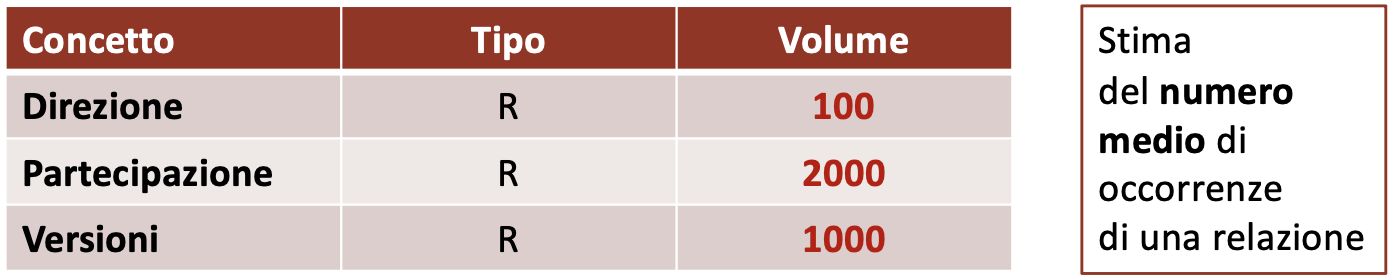
\includegraphics[width=0.6\textwidth]{foto 10.png}
\end{center}
In questo caso, le \textbf{assunzioni} possibili sono due: ogni progetto ha in media 10 \textit{release}, e ad ogni progetto lavorano in media 20 \textit{dipendenti}.\vspace*{14pt}\\
\textit{Tavola delle operazioni}\\
La \textbf{tavola delle operazioni} definisce l'\textbf{insieme delle operazioni} che devono essere implementate. Inoltre definisce la \textbf{tipologia} delle operazioni (\textbf{interattive/batch}) e la \textbf{frequenza} delle operazioni. \\
Le informazioni riguardanti le due tavole vengono fornite durante la \textbf{raccolta ed analisi dei requisiti}.\vspace*{14pt}\\
Si osservi un esempio di tavola delle operazioni:
\begin{center}
    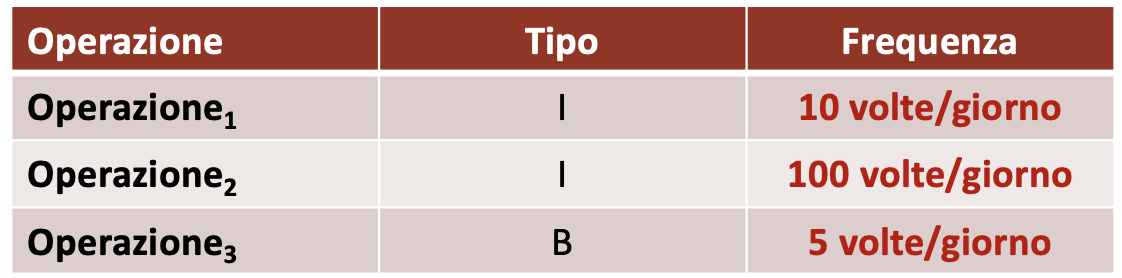
\includegraphics[width=0.6\textwidth]{foto 11.png}
\end{center}
\textbf{$Operazione_1$}: assegnare un dipendente ad un progetto\\
\textbf{$Operazione_2$}: visualizzare tutti i dati di un progetto, delle release associate e del direttore\\
\textbf{$Operazione_3$}: per ciascun progetto, visualizzare tutti i dati dei dipendenti associati\vspace{14pt}\\
Si definisce ora il concetto di \textbf{costo di una operazione}. Data un'operazione \textit{O} di tipo \textit{T}, definiamo il suo \textbf{costo c($O_T$)} come:\\
\begin{center}
    \textit{c($O_T$) = f($O_T$) $\cdot$ $w_T$ $\cdot$ ($\alpha$ $\cdot$ NCwrite + NCread)}\vspace{14pt}\\
\end{center}
Si osservi ora il glossario dei seguenti simboli:
\begin{itemize}[label={ }, leftmargin=1cm]
    \item \textit{f($O_T$)}: frequenza dell'operazione
    \item \textit{NCread}: numero di \textbf{accessi in lettura} a componenti dello schema
    \item \textit{NCwrite}: numero di \textbf{accessi in scrittura} a componenti dello schema
    \item \textit{$w_T$}: \textbf{peso} dell'operazione
    \item \textit{$\alpha$}: \textbf{coefficiente moltiplicativo} delle operazioni in scrittura\\
\end{itemize}
Tornando all'esempio delle operazioni visto in precedenza, si calcola il costo delle tre operazioni:\vspace*{14pt}\\
\textit{$Operazione_1$}\\
Assegnare un dipendente ad un progetto. La sua frequenza è di \textbf{10 volte al giorno}.
\begin{center}
    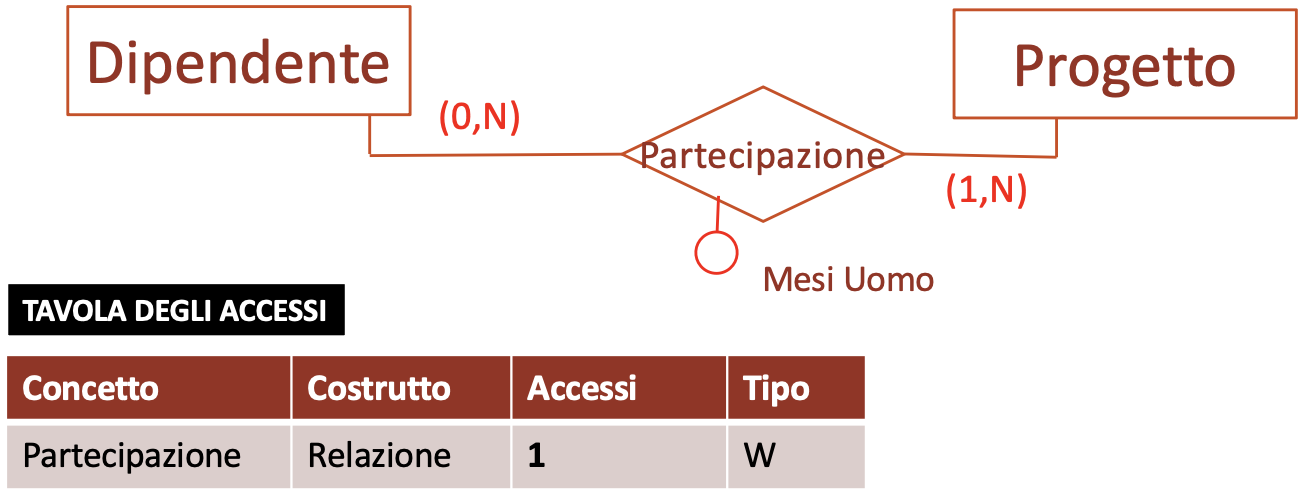
\includegraphics[width=0.6\textwidth]{foto 12.png}\vspace*{50pt}\\
\end{center}
I parametri in questo caso sono:
\begin{itemize}[label={ }, leftmargin=1cm]
    \item \textit{f($O_T$)}: 10
    \item \textit{NCread}: 0
    \item \textit{NCwrite}: 1
    \item \textit{$w_T$}: 0.5
    \item \textit{$\alpha$}: 2
\end{itemize}
Ottenendo un costo di
\begin{center}
    \textit{c(Operazione1) = 10 $\cdot$ 0.5 $\cdot$ (2 $\cdot$ 1 + 0) = 10}\vspace{14pt}\\
\end{center}
\textit{$Operazione_2$}\\
Visualizzare tutti i dati di un progetto, delle release associate e del direttore. La frequenza è di \textbf{100 volte al giorno}.
\begin{center}
    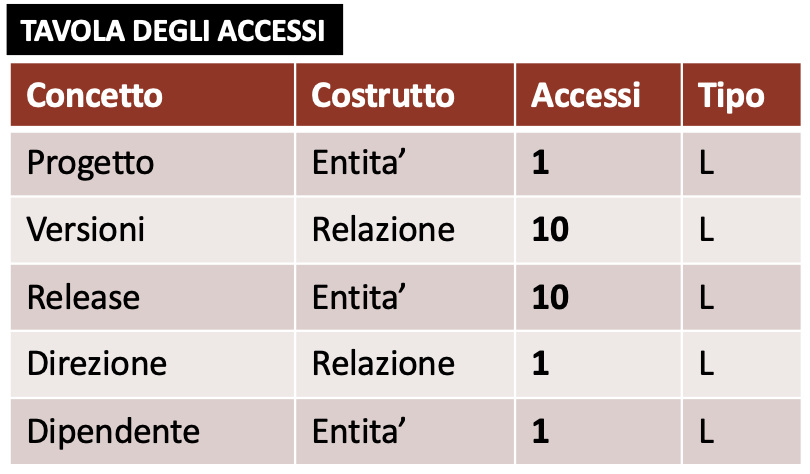
\includegraphics[width=0.5\textwidth]{foto 13.png}
\end{center}
I parametri in questo caso sono:
\begin{itemize}[label={ }, leftmargin=1cm]
    \item \textit{f($O_T$)}: 100
    \item \textit{NCread}: 23
    \item \textit{NCwrite}: 0
    \item \textit{$w_T$}: 0.5
    \item \textit{$\alpha$}: 2
\end{itemize}
Ottenendo un costo di
\begin{center}
    \textit{c(Operazione2) = 100 $\cdot$ 0.5 $\cdot$ (2 $\cdot$ 0 + 23) = 1150}\vspace{14pt}\\
\end{center}
\textit{$Operazione_3$}\\
Per ciascun progetto, visualizzare tutti i dati dei dipendenti associati. La frequenza è di \textbf{5 volte al giorno}.
\begin{center}
    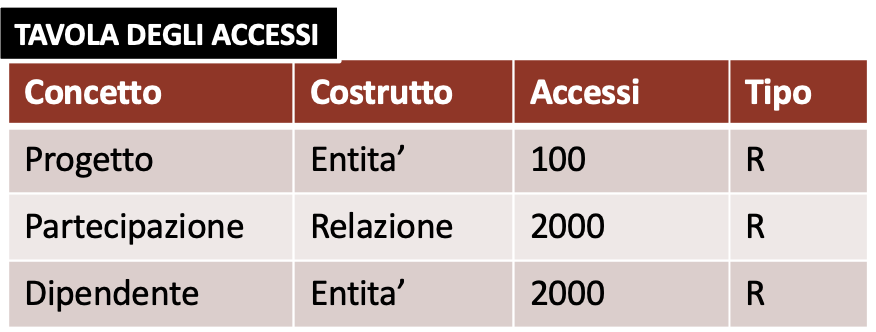
\includegraphics[width=0.5\textwidth]{foto 14.png}
\end{center}
I parametri in questo caso sono:
\begin{itemize}[label={ }, leftmargin=1cm]
    \item \textit{f($O_T$)}: 5
    \item \textit{NCread}: 4100
    \item \textit{NCwrite}: 0
    \item \textit{$w_T$}: 0.5
    \item \textit{$\alpha$}: 2
\end{itemize}
Ottenendo un costo di
\begin{center}
    \textit{c(Operazione3) = 5 $\cdot$ 0.5 $\cdot$ (2 $\cdot$ 0 + 4100) = 10250}\vspace{14pt}\\
\end{center}
Si osservi ora come calcolare il \textbf{costo dello schema} completo. Dato uno schema \textit{S}, ed un'insieme di operazioni sui dati \textit{O1, O2, \dots, On}, con costi \textit{c(O1), c(O2), c(On)}, il \textbf{costo dello schema} è definito come:\\
\begin{center}
    \textit{c(S) = $\sum_{i = 1}^{n}$ c(Oi)}\vspace{14pt}\\
\end{center}
Nell'esempio precedente si ottiene \textit{(10 + 1150 + 10250) = 11410}.\vspace*{14pt}\\
L'obiettivo del progettista è quello di \textbf{determinare lo schema E/R di costo minimo}.\\
Conoscendo la tavola dei volumi, il tipo di ciascun attributo e la sua dimensione del disco, è possibile stimare l'\textbf{occupazione di memoria dello schema}.\\
\begin{center}
    \textit{M(S) = $\sum_{entita' e}$ V(e) $\cdot$ size(e) + $\sum_{relazione r}$ V(r) $\cdot$ size(r)}\vspace{14pt}\\
\end{center}
Dove i parametri indicano:
\begin{itemize}[label={ }, leftmargin=1cm]
    \item \textit{V(e), size(e)}: tabella dei volumi e dimensione in termini di occupazione di memoria dell'entità \textit{e}
    \item \textit{V(r), size(r)}: tabella dei volumi e dimensione in termini di occupazione di memoria della relazione \textit{r}\vspace{30pt}\\
\end{itemize}
Si osservi un esempio: come stimare l'occupazione di memoria dell'entità \textit{Dipendente}.
\begin{center}
    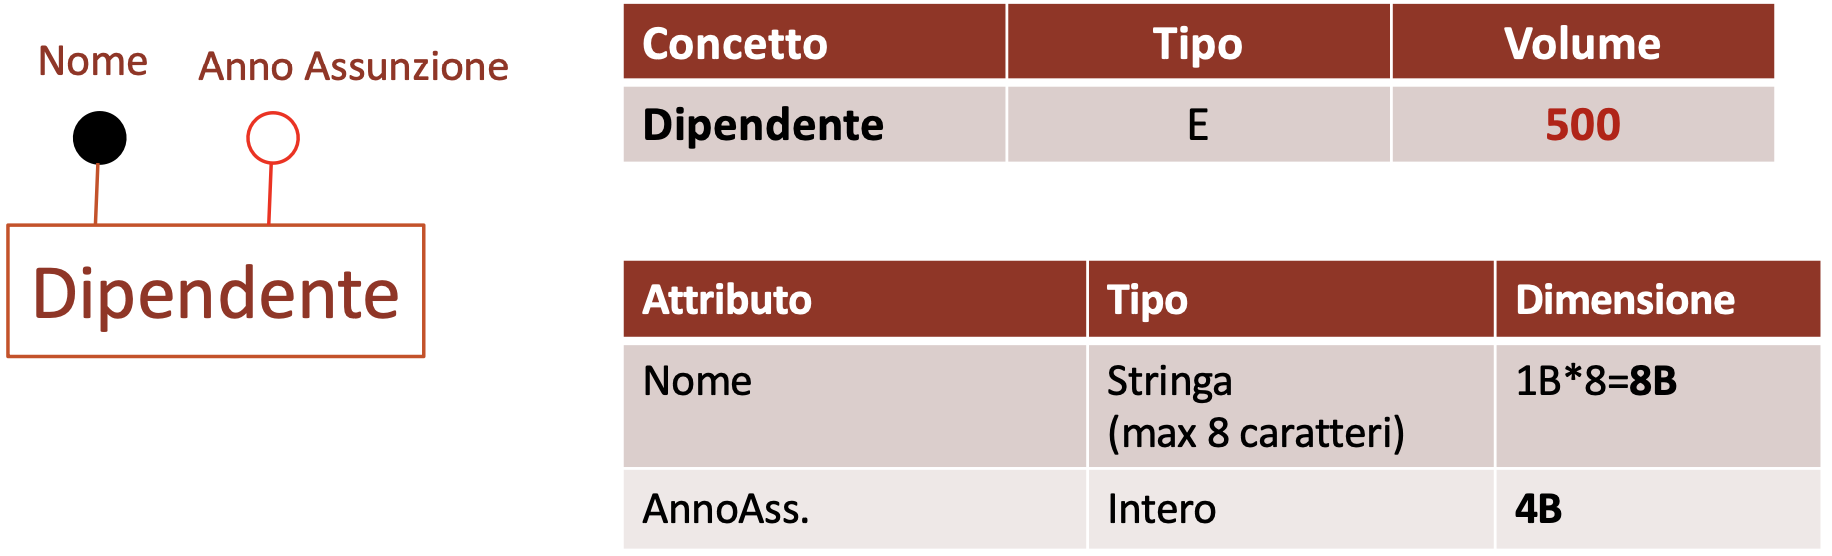
\includegraphics[width=0.6\textwidth]{foto 15.png}
\end{center}
La \textbf{Memoria Occupata} per l'entità \textit{Dipendente} è uguale a : \textit{500 * (8B + 4B) = 6000B}.\vspace{14pt}\\
In pratica, si cerca di determinare il miglior \textbf{trade-off tra occupazione di memoria e costo delle operazioni dello schema}.\\
Gli indici di prestazione di un diagramma E/R sono forniti come input alla fase di \textbf{progettazione logica}, e sono utilizzati per la \textbf{traduzione dal modello concettuale} e per l'\textbf{analisi delle ridondanze}.
\end{document}